%-------------------------------------------------------
%    DOCUMENT CONFIGURATIONS
%-------------------------------------------------------

%-------------------------------------------------------
%    START OF CRYPTOGRAPHY ANALYSE
%-------------------------------------------------------
\subsection{Cryptography}
\paragraph{Privacy} Being an integral part of Overclouds, research has been made to find the best type of client-side cryptography (right from the browser as the highest priority). We were looking for a fair middle ground between performance and security.

\subsubsection{From Scratch VS Libraries}
\paragraph{1st Question} Is it possible and does it exists right from the browser?

We started looking at what is done in JavaScript and we found an interesting list of \textit{premium} libraries (maintained by prestigious organizations) such as Stanford Javascript Crypto Library\cite{Stark2009SymmetricJavascript}, MDN\cite{MDN2015MDNCrypto}, W3C\cite{Sleevi2014WebAPI}, Google Closure\cite{Google2015ClosureLibrary}, or msrCrypto\cite{Microsoft2015MSRLibrary}.

Then we looked at other crypto libraries such as forge\cite{DigitalBazaar2016Forge}, jsHashes\cite{Johnston2015JsHashes}, crypto-browserify\cite{Tarr2013Crypto-Browserify}, etc...

\paragraph{2nd Question} The natural question that followed was: is it worth make it ourselves?

The answer came pretty quick while navigating across numerous forums. It's a pretty bad idea if we don't have a team dedicated to it and a pretty strong community to test it out. Even big companies such as Microsoft or Google are struggling a bit on the last part.

However, for the fun of it, we looked at solutions to start a homemade cryptography library. We found two interesting potential starting points to make it work with the browser, a Symmetric Encryption sample \cite{InfoTech2014SymmetricSample}, or a procedure for Digital Signatures\cite{InfoTech2014DigitalBrowser}.

\paragraph{Decision} Shortly after the second question, it was pretty clear that it will not be possible to create our cryptography library in the time given. So we decided to find the \textit{best} library out there for our project.

\subsubsection{Comparison of some JavaScript Cryptography Libraries}
\begin{table}[htpb]
\centering
\caption{Key Derivation (pbkdf2) based on figures ~\ref{fig:pbkdf2-sha1}, ~\ref{fig:pbkdf2-ops-sha1}, ~\ref{fig:pbkdf2-sha256}, ~\ref{fig:pbkdf2-ops-sha256}}
\label{tab:key-derivation-pbkdf2}
\begin{adjustbox}{center, width=\columnwidth-20pt}
\begin{tabular}{|l|l|l|l|l|}
\hline
Libraries & Sha1 (time) & Sha1 (size) & Sha256 (time) & Sha256 (size)    \\ \hline
sjcl                & \textbf{Amazing}    & \textbf{Amazing}    & \textbf{Amazing}     & \textbf{Amazing}        \\ \hline
crypto-js            & Awful    & Awful    & Awful    & Awful        \\ \hline
forge                & \textbf{Amazing}    & Nice        & \textbf{Amazing}    & Okay                \\ \hline
crypto-browserify    & \textbf{Amazing}    & Nice        & Good        & Ugly            \\ \hline
\end{tabular}
\end{adjustbox}
\end{table}

Based on the table ~\ref{tab:key-derivation-pbkdf2} below and the following referenced tables we can notice that \textbf{sjcl}\cite{Stark2009SymmetricJavascript}, \textbf{crypto browserify}\cite{Tarr2013Crypto-Browserify}, and \textbf{forge}\cite{DigitalBazaar2016Forge} algorithms have been optimized for defined objectives.

Also see Tables ~\ref{tab:hashing-0-10mb-files} and ~\ref{tab:hashing-small-files}
and their related Figures ~\ref{fig:hash-sha1}, ~\ref{fig:hash-ops-sha1}, ~\ref{fig:hash-sha256}, ~\ref{fig:hash-ops-sha256}, ~\ref{fig:small-hash-sha1}, ~\ref{fig:small-hash-sha256}

Read the table as going from Amazing to Awful.

\subsubsection{A killer}

After taking time doing research about the above algorithms, we came across a pretty amazing algorithm based on Sha3: \textbf{BLAKE2}\cite{Guo2014AnalysisBLAKE2,SaarinenM-J.2015TheMAC}.

BLAKE2 outperforms MD5, SHA-1, SHA-2, and SHA-3 on recent Intel CPUs and it has \textbf{no known} security issues. Plus SHA-1, MD5, and SHA-512 are susceptible to length-extension.

It is a \textit{new} algorithm designed specifically for \textbf{performance} and is multifaceted \textbf{BLAKE2s} (optimized for 8to32-bit) and \textbf{BLAKE2b} (optimized for 64-bit)

\subsubsection{Now what}
\begin{figure}[htpb]
\centering
\caption{\small \sl y-axis size/time, higher is better
\label{fig:hash-ops-best}}
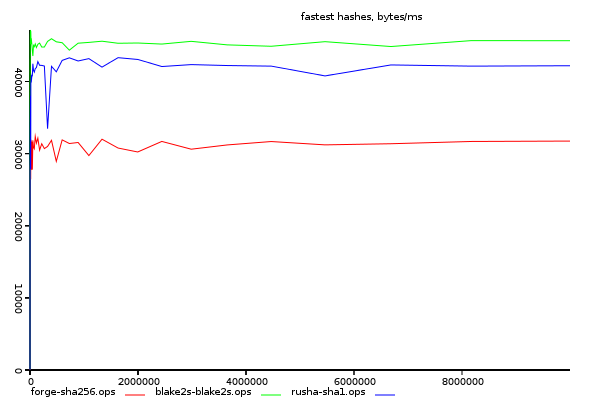
\includegraphics[scale=0.6]{annexes/graphs/hash-ops-best.png}
\end{figure} 

\begin{figure}[htpb]
\centering
\caption{\small \sl lower is better
\label{fig:blake2-sandy}}
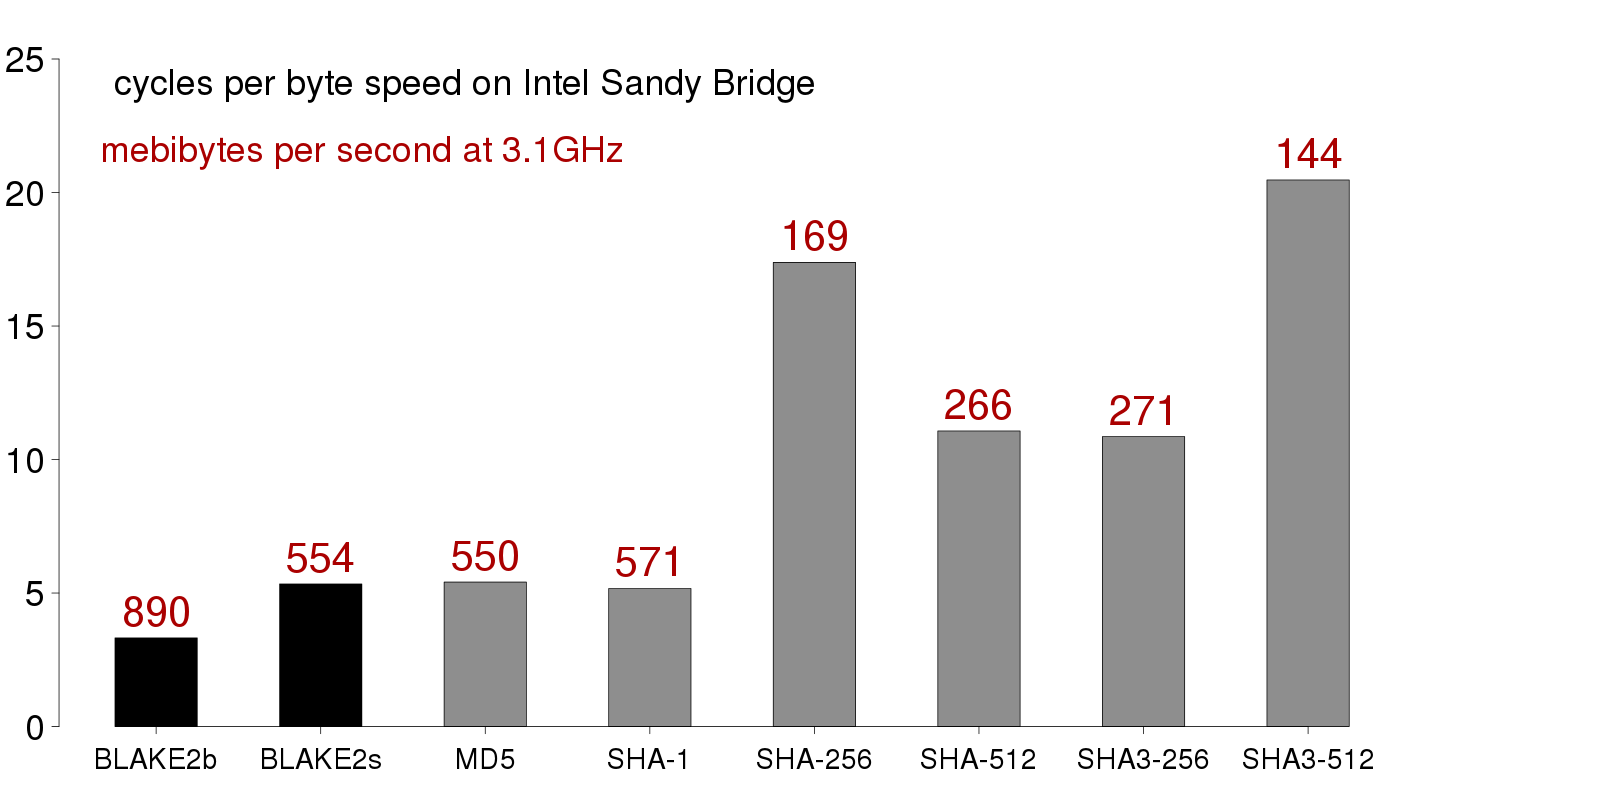
\includegraphics[scale=0.3]{annexes/graphs/blake2-sandy.png}
\end{figure}

If we look at the figure ~\ref{fig:hash-ops-best}, BLAKE2 is dominating the two best above. \textbf{rusha} is close behind it, and forge's \textit{sha256}. Plus we can note that the curves display a nearly completely linear performance.

Also on at the table ~\ref{tab:fastest-hashes} with the figure ~\ref{fig:blake2-sandy}, we notice that BLAKE2 is in its own category. 

\subsubsection{What about OverClouds}

\begin{table}[htpb]
\centering
\caption{Fastest Hashes /milliseconds based on figures ~\ref{fig:hash-ops-best}, ~\ref{fig:blake2-sandy}}
\label{tab:fastest-hashes}
\begin{adjustbox}{center, width=\columnwidth-20pt}
\begin{tabular}{|l|l|l|l|l|}
\hline
Libraries & Sha1 (size) & Sha256 (size) & Sha3 (size) \\ \hline
rusha    & \textbf{Amazing}    & Neutral    & Neutral        \\ \hline
forge    & Neutral    & \textbf{Amazing}    & Neutral        \\ \hline
blake2s    & Neutral    & Neutral    & \textbf{Amazing}    \\ \hline
\end{tabular}
\end{adjustbox}
\end{table}
We can note that we are not really interested in SHA1, because of potential security flaws. SHA256 is much better for us. However, BLACK2 is pretty amazing. We will try to make it work in the following implementation.

Now, if it doesn't work for whatever reason, we will certainly go with forge, crypto-browserify, or sjcl. The problem with forge and crypto-browserify is that we must trust a company or an individual. With sjcl however, we trust an institution.

%-------------------------------------------------------
%    END OF COMMUNICATION ANALYSE
%-------------------------------------------------------